\documentclass[11pt]{article}

\usepackage[T1]{fontenc}
\usepackage[utf8]{inputenc}
\usepackage{lmodern}
\usepackage[margin=1in]{geometry}
\usepackage{indentfirst}
\usepackage{microtype}
\usepackage{booktabs}
\usepackage{amsmath}
\usepackage{amsfonts}
\usepackage{array}
\usepackage{tabularx}
\usepackage{longtable}
\usepackage{graphicx}
\usepackage{float}
\usepackage[numbers,sort&compress]{natbib}
\usepackage{hyperref}

\hypersetup{
  colorlinks=true,
  linkcolor=blue,
  citecolor=blue,
  urlcolor=blue,
  pdftitle={Volatility Trading with Delta-Hedged ATM Straddles},
}

\title{Volatility Trading with Delta-Hedged ATM Straddles}

\makeatletter
\def\@maketitle{%
  \newpage
  \null
  \vspace*{0.75in}%
  \vskip 2em%
  \begin{center}%
    \let\footnote\thanks
    \rule{\textwidth}{4pt}\par
    \vspace{0.25in}%
    {\fontsize{17}{20}\selectfont\bfseries\@title\par}%
    \vspace{0.25in}%
    \rule{\textwidth}{1pt}\par
    \vskip 2.5em%
    {\large
      \lineskip .5em%
      \begin{tabular}[t]{c}%
        \@author
      \end{tabular}\par}%
  \end{center}%
  \vskip 1.5em
}
\makeatother

\date{}

\author{%
  Dingjingmu (Steven) Yang \\
  STAT8020: Quantitative Strategies and Algorithmic Trading\\
  Master of Data Science\\
  The University of Hong Kong\\
  \texttt{u3664645@connect.hku.hk} \\
}

\begin{document}

\maketitle

\begin{abstract}
Abstract to be completed in the final version.
\end{abstract}

\clearpage

\section{Introduction}
\label{sec:intro}

This report studies a low-frequency volatility trading strategy implemented through one-month at-the-money (ATM) straddles on U.S. equities and exchange-traded funds. The core idea is simple: options embed the market's forward-looking assessment of risk through implied volatility, while the underlying asset reveals realized volatility only after price moves occur. A persistent gap between the two creates a natural trading signal. When implied volatility appears rich relative to an appropriate benchmark, the strategy sells volatility through a short straddle; when implied volatility appears cheap, it buys volatility through a long straddle.

The key challenge is that an option position is not a pure volatility bet. A straddle carries directional sensitivity, convexity, time decay, and sensitivity to changes in interest rates and implied volatility itself. For that reason, the strategy overlays delta hedging in the underlying and evaluates performance through a daily Greeks-based attribution. The objective is not merely to report returns, but to show whether profits arise from the intended volatility exposure rather than from incidental equity direction.

The intended audience is assumed to be familiar with stocks, returns, and standard backtesting ideas, but not necessarily with option trading. The discussion therefore introduces the economic intuition of a straddle, explains the role of implied volatility and Greeks, and then presents the trading rules and empirical results in a self-contained way.

\section{Options Preliminaries}
\label{sec:pricing}

\subsection{Call, put, and straddle}

A call option gives its holder the right, but not the obligation, to buy the underlying asset at a predetermined strike price $K$ before or at expiry. A put option gives the right to sell at the same strike. The holder of a long option pays the option price upfront and has limited downside equal to that payment. The seller of the option receives that payment upfront but assumes the contingent liability.

At expiry $T$, the terminal payoffs of a call and a put are
\[
\text{Call payoff}=\max(S_T-K,0), \qquad
\text{Put payoff}=\max(K-S_T,0),
\]
where $S_T$ is the underlying price at expiry.

The strategy trades an at-the-money straddle, which is the combination of one call and one put written on the same underlying, with the same strike and the same expiry. At expiry, the payoff of a long straddle is
\[
\max(S_T-K,0)+\max(K-S_T,0)=|S_T-K|,
\]
so the position benefits from sufficiently large moves in either direction. This makes the straddle the natural vehicle for expressing a view on volatility rather than on market direction.

\begin{figure}[H]
  \centering
  \begin{minipage}{0.42\textwidth}
    \centering
    
\includegraphics[width=\linewidth]{images/pnl_call.png}
  \end{minipage}\hfill
  \begin{minipage}{0.42\textwidth}
    \centering
    
\includegraphics[width=\linewidth]{images/pnl_put.png}
  \end{minipage}
  \caption{Illustrative maturity P\&L of a long call and a long put.}
  \label{fig:call-put-pnl}
\end{figure}

\begin{figure}[H]
  \centering
  \begin{minipage}{0.42\textwidth}
    \centering
    
\includegraphics[width=\linewidth]{images/pnl_long_straddle.png}
  \end{minipage}\hfill
  \begin{minipage}{0.42\textwidth}
    \centering
    
\includegraphics[width=\linewidth]{images/pnl_short_straddle.png}
  \end{minipage}
  \caption{Illustrative maturity P\&L of long and short ATM straddles.}
  \label{fig:straddle-pnl}
\end{figure}

\subsection{Black--Scholes model}

This report uses the Black--Scholes model as the starting point for option valuation. The model provides a tractable mapping between an option's value and the key state variables that drive it: the underlying price, strike, time to maturity, risk-free rate, and volatility. Although listed equity options are American-style in legal form, Black--Scholes remains a standard and useful approximation for short-dated liquid contracts, especially when the main objective is to infer implied volatility and measure risk exposures consistently.

For a European call and put with time to maturity $\tau=T-t$, risk-free rate $r$, and volatility $\sigma$, prices are
\[
C=S_t N(d_1)-Ke^{-r\tau}N(d_2), \qquad
P=Ke^{-r\tau}N(-d_2)-S_tN(-d_1),
\]
where
\[
d_1=\frac{\ln(S_t/K)+(r+\tfrac{1}{2}\sigma^2)\tau}{\sigma\sqrt{\tau}},
\qquad
d_2=d_1-\sigma\sqrt{\tau},
\]
and $N(\cdot)$ denotes the standard normal cumulative distribution function.

\subsection{Greeks}

The value of an option depends on the underlying price, implied volatility, time to expiry, and interest rates. The Greeks summarize local sensitivities:
\[
\Delta=\frac{\partial V}{\partial S}, \qquad
\Gamma=\frac{\partial^2 V}{\partial S^2}, \qquad
\Theta=\frac{\partial V}{\partial t}, \qquad
\nu=\frac{\partial V}{\partial \sigma}, \qquad
\rho=\frac{\partial V}{\partial r},
\]
\[
\text{Vanna}=\frac{\partial^2 V}{\partial S\,\partial \sigma},
\qquad
\text{Volga}=\frac{\partial^2 V}{\partial \sigma^2}.
\]

For the present strategy, the most important interpretations are straightforward. Delta measures first-order directional exposure to the underlying. Gamma captures convexity in the underlying price. Vega measures sensitivity to changes in implied volatility. Theta represents time decay. Vanna and volga become relevant when the underlying and implied volatility move jointly or when volatility changes materially.

A second-order expansion of option value over a short interval provides the basic P\&L map:
\[
\mathrm{d}V \approx
\Delta\,\mathrm{d}S
+\frac{1}{2}\Gamma\,\mathrm{d}S^2
+\nu\,\mathrm{d}\sigma
+\Theta\,\mathrm{d}t
+\rho\,\mathrm{d}r
+\text{Vanna}\,\mathrm{d}S\,\mathrm{d}\sigma
+\frac{1}{2}\text{Volga}\,(\mathrm{d}\sigma)^2
+\varepsilon,
\]
where $\varepsilon$ captures higher-order terms. This decomposition follows the standard treatment of option risk attribution in \citet{bossu2014}. It is useful later when interpreting whether a delta-hedged straddle is actually earning volatility-related P\&L.

\subsection{Implied volatility}

Implied volatility is the value of $\sigma$ that makes the Black--Scholes price match the observed market price of an option or option package. In that sense, implied volatility is not directly observed; it is backed out from price. Practitioners often quote options in implied-volatility terms because volatility provides a standardized way to compare option richness across time and across contracts.

This interpretation is central to the strategy studied in this report. The trading decision is not driven by a view on whether the stock will rise or fall. Instead, it is driven by whether the option market appears to be charging too much or too little for future uncertainty relative to a benchmark for expected or normal volatility.

\section{Methodology}
\label{sec:methodology}

\subsection{Data}

The empirical sample consists of three exchange-traded funds, namely SPY, QQQ, and DIA, together with a set of individual U.S. equities: AAPL, ACMR, AMD, GOOG, INTC, META, and TSLA. These assets provide a useful mix of broad market exposure and single-name volatility, allowing the strategy to be examined across instruments with different liquidity conditions, sector compositions, and event risk. The individual stocks are not selected through a formal screening rule; rather, they are chosen largely at random from names with which I am personally familiar, so the single-stock sample should be interpreted as illustrative rather than exhaustive.

Although the strategy is implemented on all of these symbols, this report focuses primarily on the performance of SPY. The reason is practical as well as economic: SPY is the most popular and most liquid ETF in the sample, its options market is particularly deep, and its prices are therefore less affected by idiosyncratic microstructure noise than those of many single stocks. For that reason, SPY provides the cleanest setting for evaluating whether the strategy behaves as intended.

For each symbol and each month, the strategy selects an at-the-money straddle associated with the next monthly expiry. The strike is fixed at entry and the position is monitored through the month. As the underlying moves, the contract drifts away from exact at-the-money status; this is a deliberate simplification consistent with a low-frequency monthly trading design.

\subsubsection{Data construction details}

Each daily observation combines the underlying close, cash dividends, a short-dated risk-free rate, and the closing prices of the selected call and put. From these inputs, the dataset computes realized volatility, leg-level implied volatilities, a single straddle implied volatility that matches the observed straddle price, and the standard Greeks for both individual legs and the straddle as a whole. All volatility measures are annualized using a 252-trading-day convention.

Positions are delta hedged using the underlying. If the absolute net delta of the portfolio exceeds the re-hedging threshold, the stock hedge is adjusted and hedge shares are rounded to integers. This overlay does not remove all directional risk, but it reduces first-order exposure and makes the strategy more interpretable as a volatility trade rather than a disguised directional position.

\subsection{Trading signal}

All four agents share the same execution layer. A long-volatility position corresponds to buying one straddle, while a short-volatility position corresponds to selling one straddle when shorting is allowed. Positions are closed when the signal reverts toward its neutral region, and the hedge is updated whenever the net delta drifts beyond the chosen threshold.

\subsubsection{Realized volatility benchmark}

The classic benchmark in volatility trading is the volatility risk premium,
\[
\mathrm{VRP}_t=\mathrm{IV}_t-\mathrm{RV}_t.
\]
Here, $\mathrm{IV}_t$ denotes the implied volatility of the traded straddle and $\mathrm{RV}_t$ denotes realized volatility estimated from recent underlying returns. The intuition is direct: if implied volatility is high relative to realized volatility, the option market may be overpricing future uncertainty; if implied volatility is low relative to realized volatility, options may be relatively cheap.

Realized volatility is computed from a rolling 20-day window of daily log returns. If $r_t=\ln(S_t/S_{t-1})$, then
\[
\mathrm{RV}_{t,20}=\sqrt{252}\,\sqrt{\frac{1}{20}\sum_{i=1}^{20}(r_{t+1-i}-\bar r_t)^2},
\]
where $\bar r_t$ is the mean return over the same window.

This specification is the most familiar and transparent benchmark in the report, because it compares option-implied uncertainty with the variability recently observed in the underlying market.

\begin{figure}[H]
  \centering
  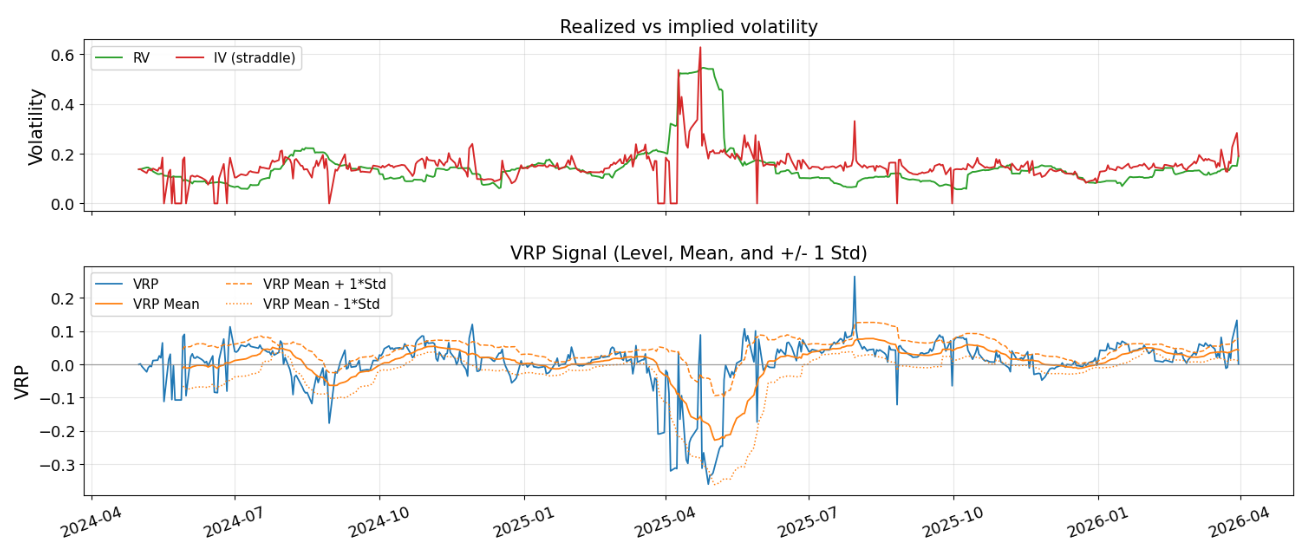
\includegraphics[width=0.92\textwidth]{images/VRP.png}
  \caption{SPY implied volatility and realized volatility in the upper panel, and the corresponding volatility risk premium in the lower panel. The lower panel also reports the rolling mean together with mean $\pm 1$ standard deviation bands.}
  \label{fig:vrp-spy}
\end{figure}

\subsubsection{GARCH-based benchmark}

The second benchmark addresses an important mismatch in a plain VRP comparison. Implied volatility reflects the market's expectation of volatility from today to option expiry, while realized volatility is computed from historical returns and does not guarantee persistence into the future. In other words, VRP compares a backward-looking statistic with a forward-looking market expectation.

To make the comparison more consistent in horizon, this benchmark replaces backward-looking realized volatility with a model-based forecast from a GJR-GARCH(1,1) specification with Student-$t$ innovations. This choice allows for volatility clustering and asymmetric responses to negative returns, both of which are common in equity data. The model is estimated on a trailing window, refit periodically, and projected forward over the remaining trading days to the option expiry.

The corresponding spread is
\[
\mathrm{IV}_t-\widehat{\mathrm{RV}}^{\mathrm{GARCH}}_t.
\]
This benchmark is designed to compare current option-implied volatility with a forward-looking conditional volatility estimate rather than with a purely historical measure.
Operationally, the signal asks whether market-implied future volatility is aligned with model-predicted future volatility.

\subsubsection{Long-horizon realized-volatility benchmark}

A third benchmark compares current straddle implied volatility with a slow-moving historical average of realized volatility. Specifically, it uses the mean of the prior 60 observations of daily realized volatility as a long-horizon anchor. The corresponding spread is therefore
\[
\mathrm{IV}_t-\overline{\mathrm{RV}}^{\mathrm{long}}_t,
\]
where $\overline{\mathrm{RV}}^{\mathrm{long}}_t$ is computed from past values only.

The economic logic is a convergence chain. Near expiry, option-implied volatility should converge to instantaneous realized volatility. A second empirical observation is that realized volatility itself tends to mean-revert. Combining these ideas gives a practical hierarchy: IV converges to RV, and RV converges to its long-horizon mean; therefore IV is expected to gravitate toward long-horizon RV as expiry approaches.

This benchmark differs conceptually from the first two. It does not compare implied volatility with the most recent realized-volatility estimate or with a model-based forecast for option expiry. Instead, it compares implied volatility with a slow-moving historical level that realized volatility itself tends to revisit over time.

\subsubsection{Z-score normalization}

The trading logic compares current straddle implied volatility with these benchmarks through a rolling 20-day z-score,
\[
Z_t(X)=\frac{X_t-\mu_{t,20}(X)}{\sigma_{t,20}(X)},
\]
where $X_t$ denotes the spread of interest and $\mu_{t,20}(X)$ and $\sigma_{t,20}(X)$ are its rolling mean and standard deviation. A sufficiently negative z-score indicates that options appear cheap relative to the benchmark, while a sufficiently positive z-score indicates that options appear expensive. This normalization makes the trading threshold comparable across different volatility regimes.

\subsubsection{Signal summary}

The implementation includes four agents built on these benchmarks. The hard-threshold rule and percentile rule both use the classic VRP idea, but they differ in how entry thresholds are defined. The GARCH-based rule replaces realized volatility with a conditional forecast. The long-horizon rule compares current implied volatility with a slow-moving historical mean of realized volatility.

\begin{table}[H]
\centering
\small
\caption{Summary of trading rules.}
\label{tab:signals}
\begin{tabularx}{\textwidth}{@{}p{0.19\textwidth}X X p{0.16\textwidth}@{}}
\toprule
Agent & Long-volatility entry & Short-volatility entry & Exit rule \\
\midrule
Hard-threshold VRP & $Z_t(\mathrm{IV}-\mathrm{RV})<-k$ & $Z_t(\mathrm{IV}-\mathrm{RV})>k$ & z-score crosses zero \\
Percentile VRP & rolling $Z_t(\mathrm{IV}-\mathrm{RV})$ in lower empirical tail & rolling $Z_t(\mathrm{IV}-\mathrm{RV})$ in upper empirical tail & z-score crosses historical median \\
GARCH spread & $Z_t(\mathrm{IV}-\widehat{\mathrm{RV}}^{\mathrm{GARCH}})<-c$ & $Z_t(\mathrm{IV}-\widehat{\mathrm{RV}}^{\mathrm{GARCH}})>c$ & z-score crosses zero \\
Long-horizon RV spread & $Z_t(\mathrm{IV}-\overline{\mathrm{RV}}^{\mathrm{long}})<-c$ & $Z_t(\mathrm{IV}-\overline{\mathrm{RV}}^{\mathrm{long}})>c$ & z-score crosses zero \\
\bottomrule
\end{tabularx}
\end{table}

The reported implementation uses the parameter settings summarized below.

\begin{table}[H]
\centering
\small
\caption{Shared execution parameters.}
\label{tab:shared-params}
\begin{tabularx}{\textwidth}{@{}p{0.28\textwidth}X p{0.16\textwidth}@{}}
\toprule
Parameter & Description & Value \\
\midrule
\texttt{allow\_short} & Whether short-volatility positions are allowed & True \\
\texttt{delta\_hedge} & Whether the straddle is hedged with the underlying & True \\
\texttt{rehedge\_threshold} & Absolute net delta that triggers hedge rebalancing & 0.05 \\
\bottomrule
\end{tabularx}
\end{table}

\begin{table}[H]
\centering
\small
\caption{Agent-specific signal parameters.}
\label{tab:agent-params}
\begin{tabularx}{\textwidth}{@{}p{0.28\textwidth}X p{0.16\textwidth}@{}}
\toprule
Agent & Parameter & Value \\
\midrule
Hard-threshold VRP & $k$ & 1.0 \\
Percentile VRP & Entry percentile & 0.20 \\
GARCH spread & Entry threshold $c$ & 1.0 \\
Long-horizon IV spread & Entry threshold $c$ & 1.0 \\
Long-horizon IV spread & Long-term RV window & 60 \\
\bottomrule
\end{tabularx}
\end{table}

All parameters are fixed before the backtest is run. They are not fitted, trained, or optimized on the in-sample period, and the same group of parameter values is applied to every underlying in the sample. This design choice is intended to limit overfitting and make the cross-asset comparison more meaningful.

\section{Results}
\label{sec:results}

\subsection{Performance on SPY}
\subsubsection{Return summary}
\begin{table}[H]
\centering
\footnotesize
\caption{SPY performance summary under updated parameter settings.}
\label{tab:spy-return-summary}
\resizebox{\textwidth}{!}{%
\begin{tabular}{lrrrrrrrr}
\toprule
Agent & Win Rate & Sharpe & Sortino & Ann. Return & Ann. Vol. & Max DD & Calmar & Kelly \\
\midrule
\texttt{Agent\_hardThreshold} & \underline{75.00\%} & \underline{1.3248} & \underline{1.1919} & \underline{25.96\%} & 17.42\% & \underline{-11.12\%} & \underline{2.3339} & \underline{7.6042} \\
\texttt{Agent\_Perc} & 74.36\% & 1.2669 & 1.1843 & 24.85\% & 17.52\% & \underline{-11.12\%} & 2.2345 & 7.2312 \\
\texttt{Agent\_Garch} & 74.47\% & 1.0765 & 0.9319 & 21.49\% & 18.09\% & -14.99\% & 1.4338 & 5.9520 \\
\texttt{Agent\_LongTerm} & 73.91\% & 1.0618 & 1.1015 & 25.56\% & \underline{21.44\%} & -11.95\% & 2.1381 & 4.9534 \\
\bottomrule
\end{tabular}%
}
\end{table}
Table~\ref{tab:spy-return-summary} summarizes risk-adjusted performance. \texttt{Agent\_hardThreshold} delivers the strongest Sharpe ratio (1.3248) and Calmar ratio (2.3339). \texttt{Agent\_Perc} is close in both return and risk metrics. \texttt{Agent\_LongTerm} achieves high annual return (25.56\%) with higher volatility (21.44\%), while \texttt{Agent\_Garch} remains profitable but with lower risk-adjusted efficiency in this run.

Figure~\ref{fig:return-curve} reports cumulative value-ratio paths (top panel) and daily return series (bottom panel) for SPY and the four strategy agents under the updated parameter set. All four agents outperform the underlying over the sample, with final value ratios clustered around 1.45--1.57 versus roughly 1.30 for SPY.

\begin{figure}[H]
  \centering
  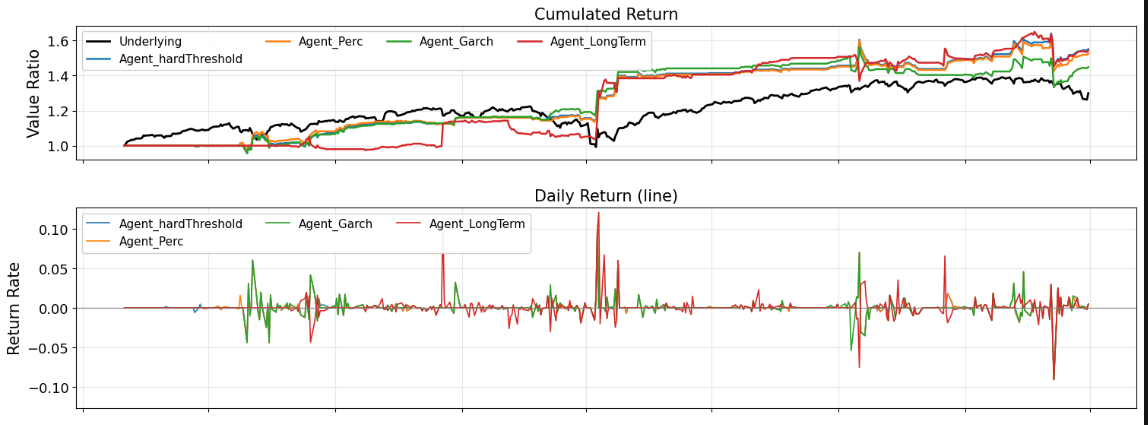
\includegraphics[width=0.96\textwidth]{images/Return_curve.png}
  \caption{SPY cumulative return (value ratio) and daily return comparison across agents.}
  \label{fig:return-curve}
\end{figure}



\subsubsection{P\&L attribution}

Daily P\&L is decomposed via a second-order Greek expansion:
\[
\mathrm{d}V \approx
\underbrace{\Delta\,\mathrm{d}S}_{\text{Delta}}
+\underbrace{\frac{1}{2}\Gamma\,\mathrm{d}S^2}_{\text{Gamma}}
+\underbrace{\nu\,\mathrm{d}\sigma}_{\text{Vega}}
+\underbrace{\Theta\,\mathrm{d}t}_{\text{Theta}}
+\underbrace{\rho\,\mathrm{d}r}_{\text{Rho}}
+\underbrace{\text{Vanna}\,\mathrm{d}S\,\mathrm{d}\sigma}_{\text{Vanna}}
+\underbrace{\frac{1}{2}\text{Volga}\,(\mathrm{d}\sigma)^2}_{\text{Volga}}
+\varepsilon.
\]
The P\&L from delta re-hedging trades is merged into the Gamma term, so the Gamma attribution captures both the convexity gain and the realized cost or benefit of maintaining the hedge.

For each Greek component $i$, the reported percentage contribution is computed as
\[
\text{Greek \%}_i=
\frac{\text{Greek}_i\text{ summed attribution}}
{\sum_j \left|\text{Greek}_j\text{ summed attribution}\right|}
\times 100.
\]

Figure~\ref{fig:greeks-attribution} shows the summed attribution breakdown for each agent. Vega is the dominant P\&L source across all strategies, confirming that returns are primarily driven by volatility mispricing rather than directional exposure. Notably, \texttt{Agent\_LongTerm} records the highest vega attribution (58.2\%), indicating that the long-horizon realized-volatility signal is the most effective at capturing volatility mispricing and benefiting from implied volatility mean-reversion.

\begin{figure}[H]
  \centering
  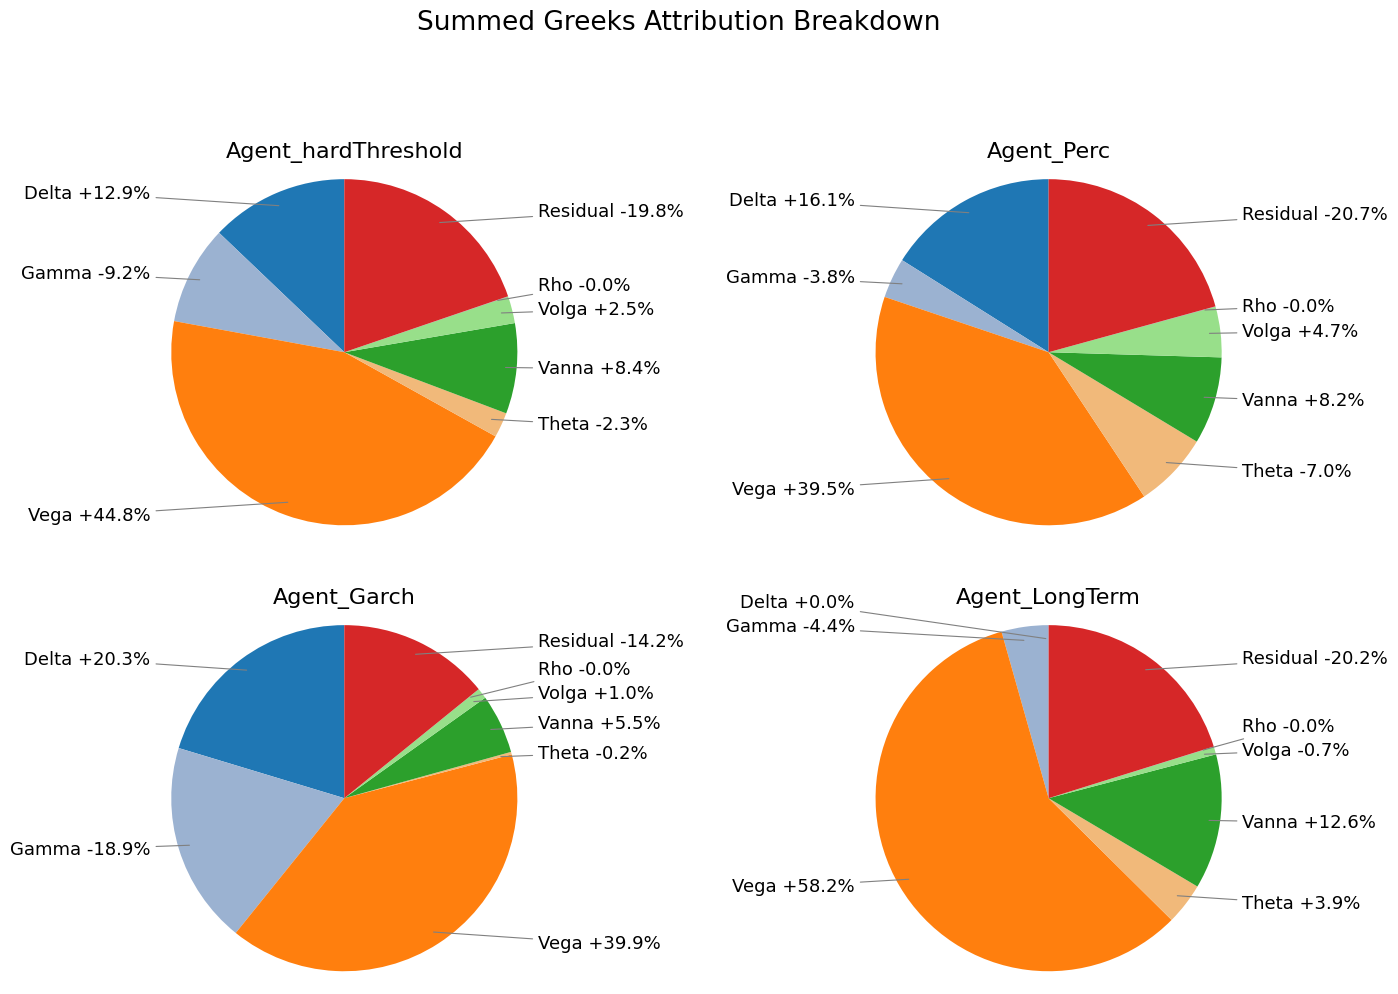
\includegraphics[width=0.85\textwidth]{images/Greeks_attribution.png}
  \caption{Summed Greeks attribution breakdown by strategy agent on SPY.}
  \label{fig:greeks-attribution}
\end{figure}

\subsection{Performance on other ETFs}

Table~\ref{tab:etf-return-summary} reports performance statistics for QQQ and DIA under the same parameter set used in the SPY section. DIA is stronger on a risk-adjusted basis across agents (higher Sharpe and Sortino), while QQQ remains profitable but with larger drawdowns and more dispersion across agents.

\begin{table}[H]
\centering
\footnotesize
\caption{QQQ and DIA performance summary by agent.}
\label{tab:etf-return-summary}
\resizebox{\textwidth}{!}{%
\begin{tabular}{llrrrrrr}
\toprule
Ticker & Agent & Win Rate & Sharpe & Sortino & Ann. Return & Ann. Vol. & Max DD \\
\midrule
QQQ & \texttt{Agent\_hardThreshold} & \underline{81.08\%} & 0.8870 & 0.6754 & 21.10\% & 21.58\% & -20.95\% \\
QQQ & \texttt{Agent\_Perc}          & 69.23\% & 0.9749 & 1.2191 & 34.63\% & \underline{30.50\%} & -22.95\% \\
QQQ & \texttt{Agent\_Garch}         & 76.32\% & 1.1106 & 0.9158 & 28.83\% & 22.81\% & -19.81\% \\
QQQ & \texttt{Agent\_LongTerm}      & 80.00\% & \underline{1.7709} & \underline{1.5282} & \underline{46.30\%} & 21.48\% & \underline{-14.83\%} \\
\midrule
DIA & \texttt{Agent\_hardThreshold} & \underline{87.50\%} & 1.5611 & 1.2112 & 47.21\% & 24.77\% & -20.59\% \\
DIA & \texttt{Agent\_Perc}          & 87.04\% & \underline{2.2303} & \underline{2.2453} & \underline{91.18\%} & 29.06\% & \underline{-18.77\%} \\
DIA & \texttt{Agent\_Garch}         & 85.45\% & 1.9131 & 1.7752 & 68.01\% & 27.12\% & -18.97\% \\
DIA & \texttt{Agent\_LongTerm}      & 85.71\% & 2.0476 & 1.7590 & 81.61\% & \underline{29.14\%} & -19.89\% \\
\bottomrule
\end{tabular}%
}
\end{table}

Table~\ref{tab:etf-greeks-attribution} reports summed Greek attribution percentages. Across QQQ and DIA, Vega is the largest positive contributor in every agent, consistent with a volatility-risk-premium strategy. The strongest Vega attribution appears in \texttt{Agent\_LongTerm} for both ETFs (QQQ: +57.72\%, DIA: +66.42\%), indicating that this signal captures volatility-premium exposure most directly in the ETF sample. Residual attribution is generally negative, indicating that a non-trivial share of realized P\&L is outside the low-order Greek decomposition.

\begin{table}[H]
\centering
\footnotesize
\caption{QQQ and DIA Greeks attribution percentages by agent.}
\label{tab:etf-greeks-attribution}
\resizebox{\textwidth}{!}{%
\begin{tabular}{llrrrrrrrr}
\toprule
Ticker & Agent & Delta & Gamma & Vega & Theta & Vanna & Volga & Rho & Residual \\
\midrule
QQQ & \texttt{Agent\_hardThreshold} & +2.81\% & -12.76\% & +54.67\% & -0.76\% & +2.73\% & +9.64\% & +0.00\% & -16.62\% \\
QQQ & \texttt{Agent\_Perc}          & \underline{+10.38\%} & \underline{+9.51\%}  & +19.51\% & -12.03\% & \underline{+6.83\%} & \underline{+15.87\%} & -0.00\% & -25.88\% \\
QQQ & \texttt{Agent\_Garch}         & -5.33\% & +8.92\%  & +47.41\% & -6.11\% & +2.40\% & +9.83\% & +0.01\% & -19.98\% \\
QQQ & \texttt{Agent\_LongTerm}      & -0.77\% & -19.46\% & \underline{+57.72\%} & \underline{+3.42\%} & +2.34\% & +7.13\% & \underline{+0.02\%} & \underline{-9.14\%} \\
\midrule
DIA & \texttt{Agent\_hardThreshold} & -4.10\% & +3.97\%  & +48.70\% & -10.06\% & \underline{+6.17\%} & +14.41\% & +0.00\% & -12.58\% \\
DIA & \texttt{Agent\_Perc}          & \underline{-3.75\%} & +2.60\%  & +50.89\% & -8.11\% & +4.56\% & \underline{+16.20\%} & -0.00\% & -13.88\% \\
DIA & \texttt{Agent\_Garch}         & -8.63\% & \underline{+6.18\%}  & +58.07\% & -8.56\% & +2.44\% & +9.69\% & +0.00\% & \underline{-6.43\%} \\
DIA & \texttt{Agent\_LongTerm}      & -6.71\% & +1.86\%  & \underline{+66.42\%} & \underline{+0.11\%} & +1.02\% & +7.41\% & \underline{+0.01\%} & -16.46\% \\
\bottomrule
\end{tabular}%
}
\end{table}


\subsection{Performance on single stocks}

Single-stock results are more heterogeneous than ETF results, reflecting larger idiosyncratic risk and event sensitivity. In terms of risk-adjusted performance, outcomes differ substantially by ticker: for example, GOOG and INTC are strong across multiple agents, whereas AMD and parts of ACMR/META are weaker or unstable in this sample.

From a Greeks-attribution perspective, Vega remains the dominant positive component in most ticker-agent combinations. The highest Vega attribution in the single-stock panel is \texttt{Agent\_Garch} on ACMR (+67.53\%), while \texttt{Agent\_LongTerm} also shows very high Vega share on INTC (+42.03\%) and TSLA (+41.71\%). This supports the same core interpretation as in ETFs: realized strategy P\&L is primarily tied to volatility exposure, with residual and cross-greek terms explaining the remainder.

The full single-stock statistics and Greeks-attribution tables are reported in Appendix~\ref{app:single-stock-full-tables}.

\subsection{Robustness}
The cross-asset results indicate that the long-horizon realized-volatility spread is the most robust signal in this study. Using one fixed parameter set (without ticker-specific tuning), it delivers the most consistent risk-adjusted performance across SPY, QQQ, and DIA, with mixed but still competitive outcomes in several single stocks.

Greeks attribution is aligned with this conclusion: Vega is the dominant positive contributor in most cases, indicating that returns are primarily coming from volatility mispricing rather than directional beta.

Robustness is stronger in ETFs than in single names, likely because ETFs have better liquidity and lower idiosyncratic jump risk. Main limitations are sample length, execution/transaction-cost assumptions, and residual terms outside the low-order Greeks decomposition.



\section{Discussion}






\clearpage



\small
\begin{thebibliography}{9}

\bibitem[Bossu(2014)]{bossu2014}
Bossu, S\'ebastien (2014).
\emph{Advanced Equity Derivatives: Volatility and Correlation}.
Wiley Finance Series, John Wiley \& Sons, Inc., Hoboken, NJ.

\end{thebibliography}



\clearpage
\appendix
\addcontentsline{toc}{section}{Appendix}

\section{Full Single-Stock Tables}
\label{app:single-stock-full-tables}

Table~\ref{tab:stock-return-full} and Table~\ref{tab:stock-greeks-full} provide the complete single-stock results used to summarize this subsection.

\begingroup
\scriptsize
\setlength{\tabcolsep}{4pt}
\begin{longtable}{llrrrrrr}
\caption{Full single-stock performance statistics by ticker and agent.}\label{tab:stock-return-full} \\
\toprule
Ticker & Agent & Win Rate & Sharpe & Sortino & Ann. Return & Ann. Vol. & Max DD \\
\midrule
\endfirsthead

\toprule
Ticker & Agent & Win Rate & Sharpe & Sortino & Ann. Return & Ann. Vol. & Max DD \\
\midrule
\endhead

AAPL & \texttt{Agent\_hardThreshold} & 73.17\% & 0.3969 & 0.2537 & 8.21\% & 19.88\% & -21.25\% \\
AAPL & \texttt{Agent\_Perc}          & 72.22\% & 0.1404 & 0.0941 & 2.95\% & \underline{20.74\%} & -26.44\% \\
AAPL & \texttt{Agent\_Garch}         & 73.33\% & 0.1402 & 0.0891 & 2.87\% & 20.16\% & -23.40\% \\
AAPL & \texttt{Agent\_LongTerm}      & \underline{86.67\%} & \underline{0.5435} & \underline{0.3926} & \underline{9.08\%} & 15.99\% & \underline{-16.86\%} \\
\midrule
ACMR & \texttt{Agent\_hardThreshold} & 55.56\% & -0.0069 & -0.0065 & -0.27\% & 39.16\% & \underline{-25.42\%} \\
ACMR & \texttt{Agent\_Perc}          & \underline{61.54\%} & \underline{0.5744} & \underline{0.5040} & \underline{58.52\%} & \underline{80.20\%} & -32.10\% \\
ACMR & \texttt{Agent\_Garch}         & 60.00\% & 0.4892 & 0.4964 & 24.98\% & 45.58\% & -31.94\% \\
ACMR & \texttt{Agent\_LongTerm}      & 60.00\% & -0.9640 & -0.4432 & -48.66\% & 69.16\% & -42.17\% \\
\midrule
AMD  & \texttt{Agent\_hardThreshold} & 71.43\% & -0.4379 & -0.2366 & -26.84\% & \underline{71.39\%} & -65.30\% \\
AMD  & \texttt{Agent\_Perc}          & 64.71\% & -0.4454 & -0.2423 & -27.12\% & 71.04\% & -66.78\% \\
AMD  & \texttt{Agent\_Garch}         & 71.11\% & -0.4153 & -0.2214 & -25.64\% & 71.35\% & -63.65\% \\
AMD  & \texttt{Agent\_LongTerm}      & \underline{85.71\%} & \underline{-0.0922} & \underline{-0.0424} & \underline{-6.12\%} & 68.56\% & \underline{-59.33\%} \\
\midrule
GOOG & \texttt{Agent\_hardThreshold} & 79.49\% & \underline{1.6039} & 1.9659 & 58.84\% & 28.85\% & \underline{-11.57\%} \\
GOOG & \texttt{Agent\_Perc}          & \underline{81.58\%} & 1.1861 & 1.3496 & 50.25\% & \underline{34.32\%} & -16.75\% \\
GOOG & \texttt{Agent\_Garch}         & 72.09\% & 1.5513 & \underline{2.0530} & \underline{62.73\%} & 31.39\% & \underline{-11.57\%} \\
GOOG & \texttt{Agent\_LongTerm}      & 76.32\% & 0.9161 & 1.0031 & 32.45\% & 30.68\% & -22.61\% \\
\midrule
INTC & \texttt{Agent\_hardThreshold} & \underline{77.50\%} & \underline{1.4840} & 2.3184 & 124.20\% & 54.40\% & -29.63\% \\
INTC & \texttt{Agent\_Perc}          & 71.05\% & 1.3589 & \underline{2.8220} & 108.55\% & 54.09\% & \underline{-24.79\%} \\
INTC & \texttt{Agent\_Garch}         & 72.00\% & \underline{1.4840} & 2.3462 & \underline{129.95\%} & \underline{56.11\%} & -27.41\% \\
INTC & \texttt{Agent\_LongTerm}      & 76.09\% & 1.0758 & 0.9528 & 47.21\% & 35.94\% & -28.73\% \\
\midrule
META & \texttt{Agent\_hardThreshold} & \underline{65.79\%} & -0.1857 & -0.1634 & -5.96\% & 33.10\% & -32.14\% \\
META & \texttt{Agent\_Perc}          & 65.00\% & -0.3303 & -0.2649 & -9.86\% & 31.41\% & -36.48\% \\
META & \texttt{Agent\_Garch}         & \underline{65.79\%} & \underline{0.1389} & \underline{0.1267} & \underline{4.79\%} & \underline{33.72\%} & -28.72\% \\
META & \texttt{Agent\_LongTerm}      & 58.33\% & -0.0927 & -0.0777 & -2.67\% & 29.20\% & \underline{-24.03\%} \\
\midrule
TSLA & \texttt{Agent\_hardThreshold} & 68.89\% & \underline{0.7805} & \underline{0.7674} & \underline{29.31\%} & \underline{32.93\%} & -25.02\% \\
TSLA & \texttt{Agent\_Perc}          & 63.64\% & 0.5477 & 0.5530 & 18.19\% & 30.51\% & -27.21\% \\
TSLA & \texttt{Agent\_Garch}         & 71.43\% & 0.7275 & 0.7003 & 23.56\% & 29.08\% & -23.68\% \\
TSLA & \texttt{Agent\_LongTerm}      & \underline{72.34\%} & 0.1001 & 0.0701 & 2.23\% & 21.99\% & \underline{-20.69\%} \\
\bottomrule
\end{longtable}
\endgroup

\begingroup
\scriptsize
\setlength{\tabcolsep}{4pt}
\begin{longtable}{llrrrrrrrr}
\caption{Full single-stock Greeks attribution percentages by ticker and agent.}\label{tab:stock-greeks-full} \\
\toprule
Ticker & Agent & Delta & Gamma & Vega & Theta & Vanna & Volga & Rho & Residual \\
\midrule
\endfirsthead

\toprule
Ticker & Agent & Delta & Gamma & Vega & Theta & Vanna & Volga & Rho & Residual \\
\midrule
\endhead

AAPL & \texttt{Agent\_hardThreshold} & \underline{+17.52\%} & -30.20\% & +26.97\% & \underline{+10.41\%} & +3.20\% & -1.70\% & -0.01\% & \underline{-9.99\%} \\
AAPL & \texttt{Agent\_Perc}          & +9.52\%  & -11.16\% & +21.49\% & +5.86\%  & \underline{+4.14\%} & \underline{+15.59\%} & -0.01\% & -32.22\% \\
AAPL & \texttt{Agent\_Garch}         & +9.79\%  & -21.20\% & +28.28\% & +8.64\%  & +3.17\% & +7.35\%  & -0.00\% & -21.56\% \\
AAPL & \texttt{Agent\_LongTerm}      & +10.77\% & \underline{-8.78\%}  & \underline{+46.82\%} & -1.95\%  & +1.41\% & -1.72\%  & \underline{+0.00\%} & -28.56\% \\
\midrule
ACMR & \texttt{Agent\_hardThreshold} & +6.44\%  & -7.34\%  & +55.56\% & -8.52\%  & +1.03\% & \underline{+1.92\%}  & +0.00\% & -19.19\% \\
ACMR & \texttt{Agent\_Perc}          & \underline{+23.47\%} & -6.99\%  & +48.71\% & \underline{-6.22\%}  & -6.62\% & -4.91\%  & +0.02\% & \underline{-3.07\%} \\
ACMR & \texttt{Agent\_Garch}         & -7.58\%  & +6.03\%  & \underline{+67.53\%} & -6.54\%  & +1.89\% & +1.11\%  & +0.02\% & -9.31\% \\
ACMR & \texttt{Agent\_LongTerm}      & -1.19\%  & \underline{+36.75\%} & +5.91\%  & -15.02\% & \underline{+10.63\%} & -9.47\% & \underline{+0.06\%} & -20.97\% \\
\midrule
AMD  & \texttt{Agent\_hardThreshold} & +7.15\%  & -21.53\% & +8.63\%  & \underline{+8.58\%}  & +3.72\% & +25.47\% & \underline{+0.00\%} & -24.91\% \\
AMD  & \texttt{Agent\_Perc}          & +6.02\%  & \underline{-13.35\%} & +8.19\%  & +4.76\%  & \underline{+5.05\%} & \underline{+30.28\%} & \underline{-0.00\%} & -32.35\% \\
AMD  & \texttt{Agent\_Garch}         & \underline{+8.88\%}  & -22.23\% & +13.71\% & +7.24\%  & +4.27\% & +20.53\% & \underline{+0.00\%} & -23.15\% \\
AMD  & \texttt{Agent\_LongTerm}      & -5.72\%  & -13.49\% & \underline{+50.14\%} & +5.77\%  & -1.82\% & +7.03\%  & \underline{+0.00\%} & \underline{-16.03\%} \\
\midrule
GOOG & \texttt{Agent\_hardThreshold} & +12.85\% & -18.27\% & +21.75\% & \underline{+13.61\%} & -1.79\% & +11.25\% & \underline{-0.01\%} & \underline{-20.46\%} \\
GOOG & \texttt{Agent\_Perc}          & +11.50\% & \underline{-2.96\%}  & +24.81\% & +2.14\%  & -1.25\% & \underline{+20.70\%} & \underline{-0.01\%} & -36.61\% \\
GOOG & \texttt{Agent\_Garch}         & +14.37\% & -15.67\% & +19.82\% & +9.32\%  & +0.16\% & +14.76\% & \underline{-0.01\%} & -25.89\% \\
GOOG & \texttt{Agent\_LongTerm}      & \underline{+17.89\%} & -2.98\%  & \underline{+26.98\%} & +3.76\%  & \underline{+0.17\%} & +11.49\% & \underline{-0.01\%} & -36.71\% \\
\midrule
INTC & \texttt{Agent\_hardThreshold} & -5.17\%  & +7.87\%  & +20.40\% & \underline{+10.16\%} & +2.78\% & +20.65\% & \underline{-0.00\%} & -32.97\% \\
INTC & \texttt{Agent\_Perc}          & \underline{+5.30\%}  & \underline{+11.22\%} & +14.44\% & -1.52\%  & +3.31\% & \underline{+24.23\%} & \underline{-0.00\%} & -39.98\% \\
INTC & \texttt{Agent\_Garch}         & +0.85\%  & -0.51\%  & +31.48\% & +8.82\%  & +4.69\% & +16.82\% & \underline{-0.00\%} & -36.82\% \\
INTC & \texttt{Agent\_LongTerm}      & -10.42\% & +10.34\% & \underline{+42.03\%} & +3.15\%  & \underline{+5.71\%} & +3.51\%  & \underline{-0.00\%} & \underline{-24.83\%} \\
\midrule
META & \texttt{Agent\_hardThreshold} & -19.06\% & -24.77\% & +9.40\%  & +27.99\% & +0.25\% & -3.99\%  & \underline{+0.02\%} & \underline{+14.53\%} \\
META & \texttt{Agent\_Perc}          & -26.31\% & \underline{-20.21\%} & \underline{+26.12\%} & +9.76\%  & +0.01\% & \underline{+16.33\%} & \underline{+0.02\%} & -1.24\% \\
META & \texttt{Agent\_Garch}         & -17.56\% & -27.06\% & +9.44\%  & \underline{+33.54\%} & -0.02\% & +0.73\%  & +0.01\% & +11.65\% \\
META & \texttt{Agent\_LongTerm}      & \underline{+6.50\%}  & -48.47\% & +10.06\% & +22.45\% & \underline{+2.51\%} & +2.28\%  & +0.00\% & +7.72\% \\
\midrule
TSLA & \texttt{Agent\_hardThreshold} & \underline{+5.24\%}  & -13.41\% & +50.83\% & \underline{+2.63\%}  & +2.89\% & -24.38\% & \underline{+0.00\%} & \underline{+0.61\%} \\
TSLA & \texttt{Agent\_Perc}          & +1.06\%  & \underline{+10.34\%} & +32.66\% & -10.97\% & +2.58\% & \underline{+8.57\%}  & \underline{+0.00\%} & -33.79\% \\
TSLA & \texttt{Agent\_Garch}         & -2.72\%  & +1.94\%  & \underline{+53.48\%} & -4.59\%  & +3.01\% & +1.40\%  & \underline{+0.00\%} & -32.85\% \\
TSLA & \texttt{Agent\_LongTerm}      & -11.85\% & +5.65\%  & +41.71\% & -3.36\%  & \underline{+3.69\%} & +5.16\%  & \underline{-0.00\%} & -28.58\% \\
\bottomrule
\end{longtable}
\endgroup

\section{Greeks Attribution: Dollar P\&L Time Series}
\label{app:greeks-line-raw}

Figure~\ref{fig:greeks-line-raw} shows the daily dollar P\&L contribution of each Greek component across the full backtest period. Each panel corresponds to one strategy agent and breaks down the daily total P\&L into delta, gamma, vega, theta, vanna, volga, rho, and residual buckets. The time series view complements the pie chart by revealing when and for how long each risk factor dominated, and where attribution spikes occurred.

\begin{figure}[H]
  \centering
  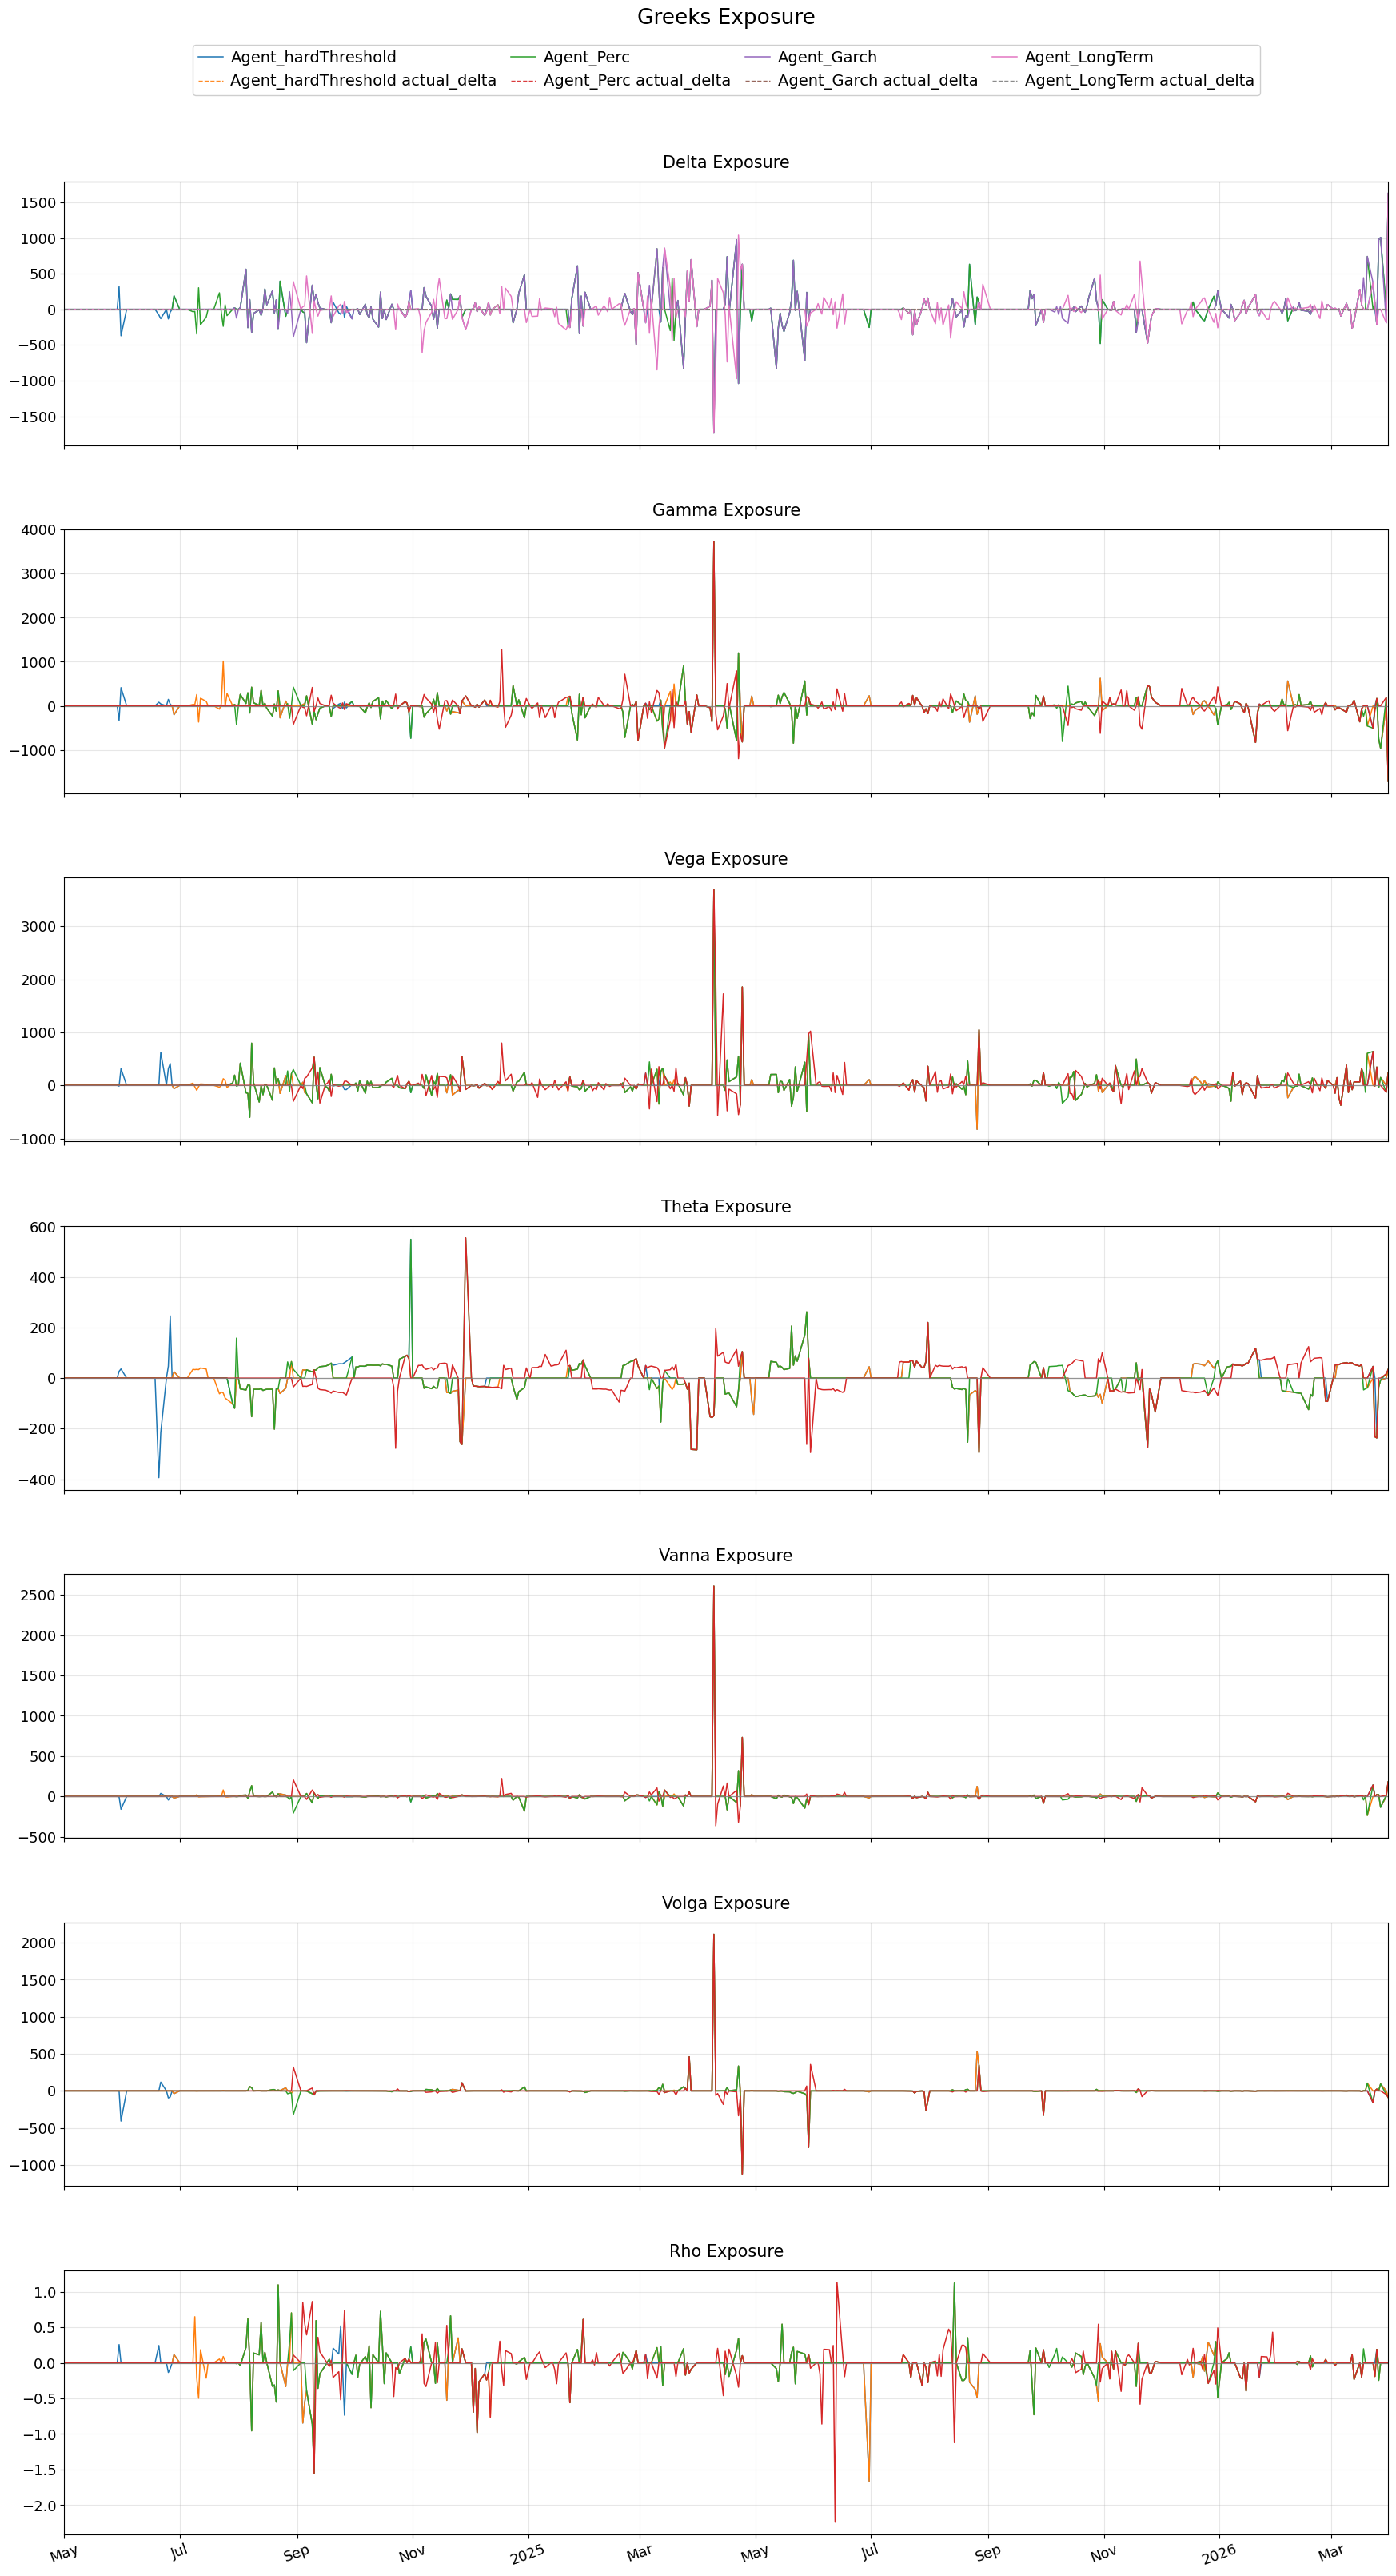
\includegraphics[width=0.70\textwidth]{images/greeks_line_raw.png}
  \caption{Daily dollar P\&L attribution by Greek component for each agent on SPY.}
  \label{fig:greeks-line-raw}
\end{figure}

\section{Greeks Exposure Over Time}
\label{app:greeks-line}

Figure~\ref{fig:greeks-line} shows the evolution of Greeks exposure over the backtest period. Unlike the dollar attribution series, this plot tracks the raw sensitivity levels (e.g.\ net vega, net delta, net gamma) as the position changes, providing insight into how risk exposures build up and unwind across entry, holding, and exit phases.

\begin{figure}[H]
  \centering
  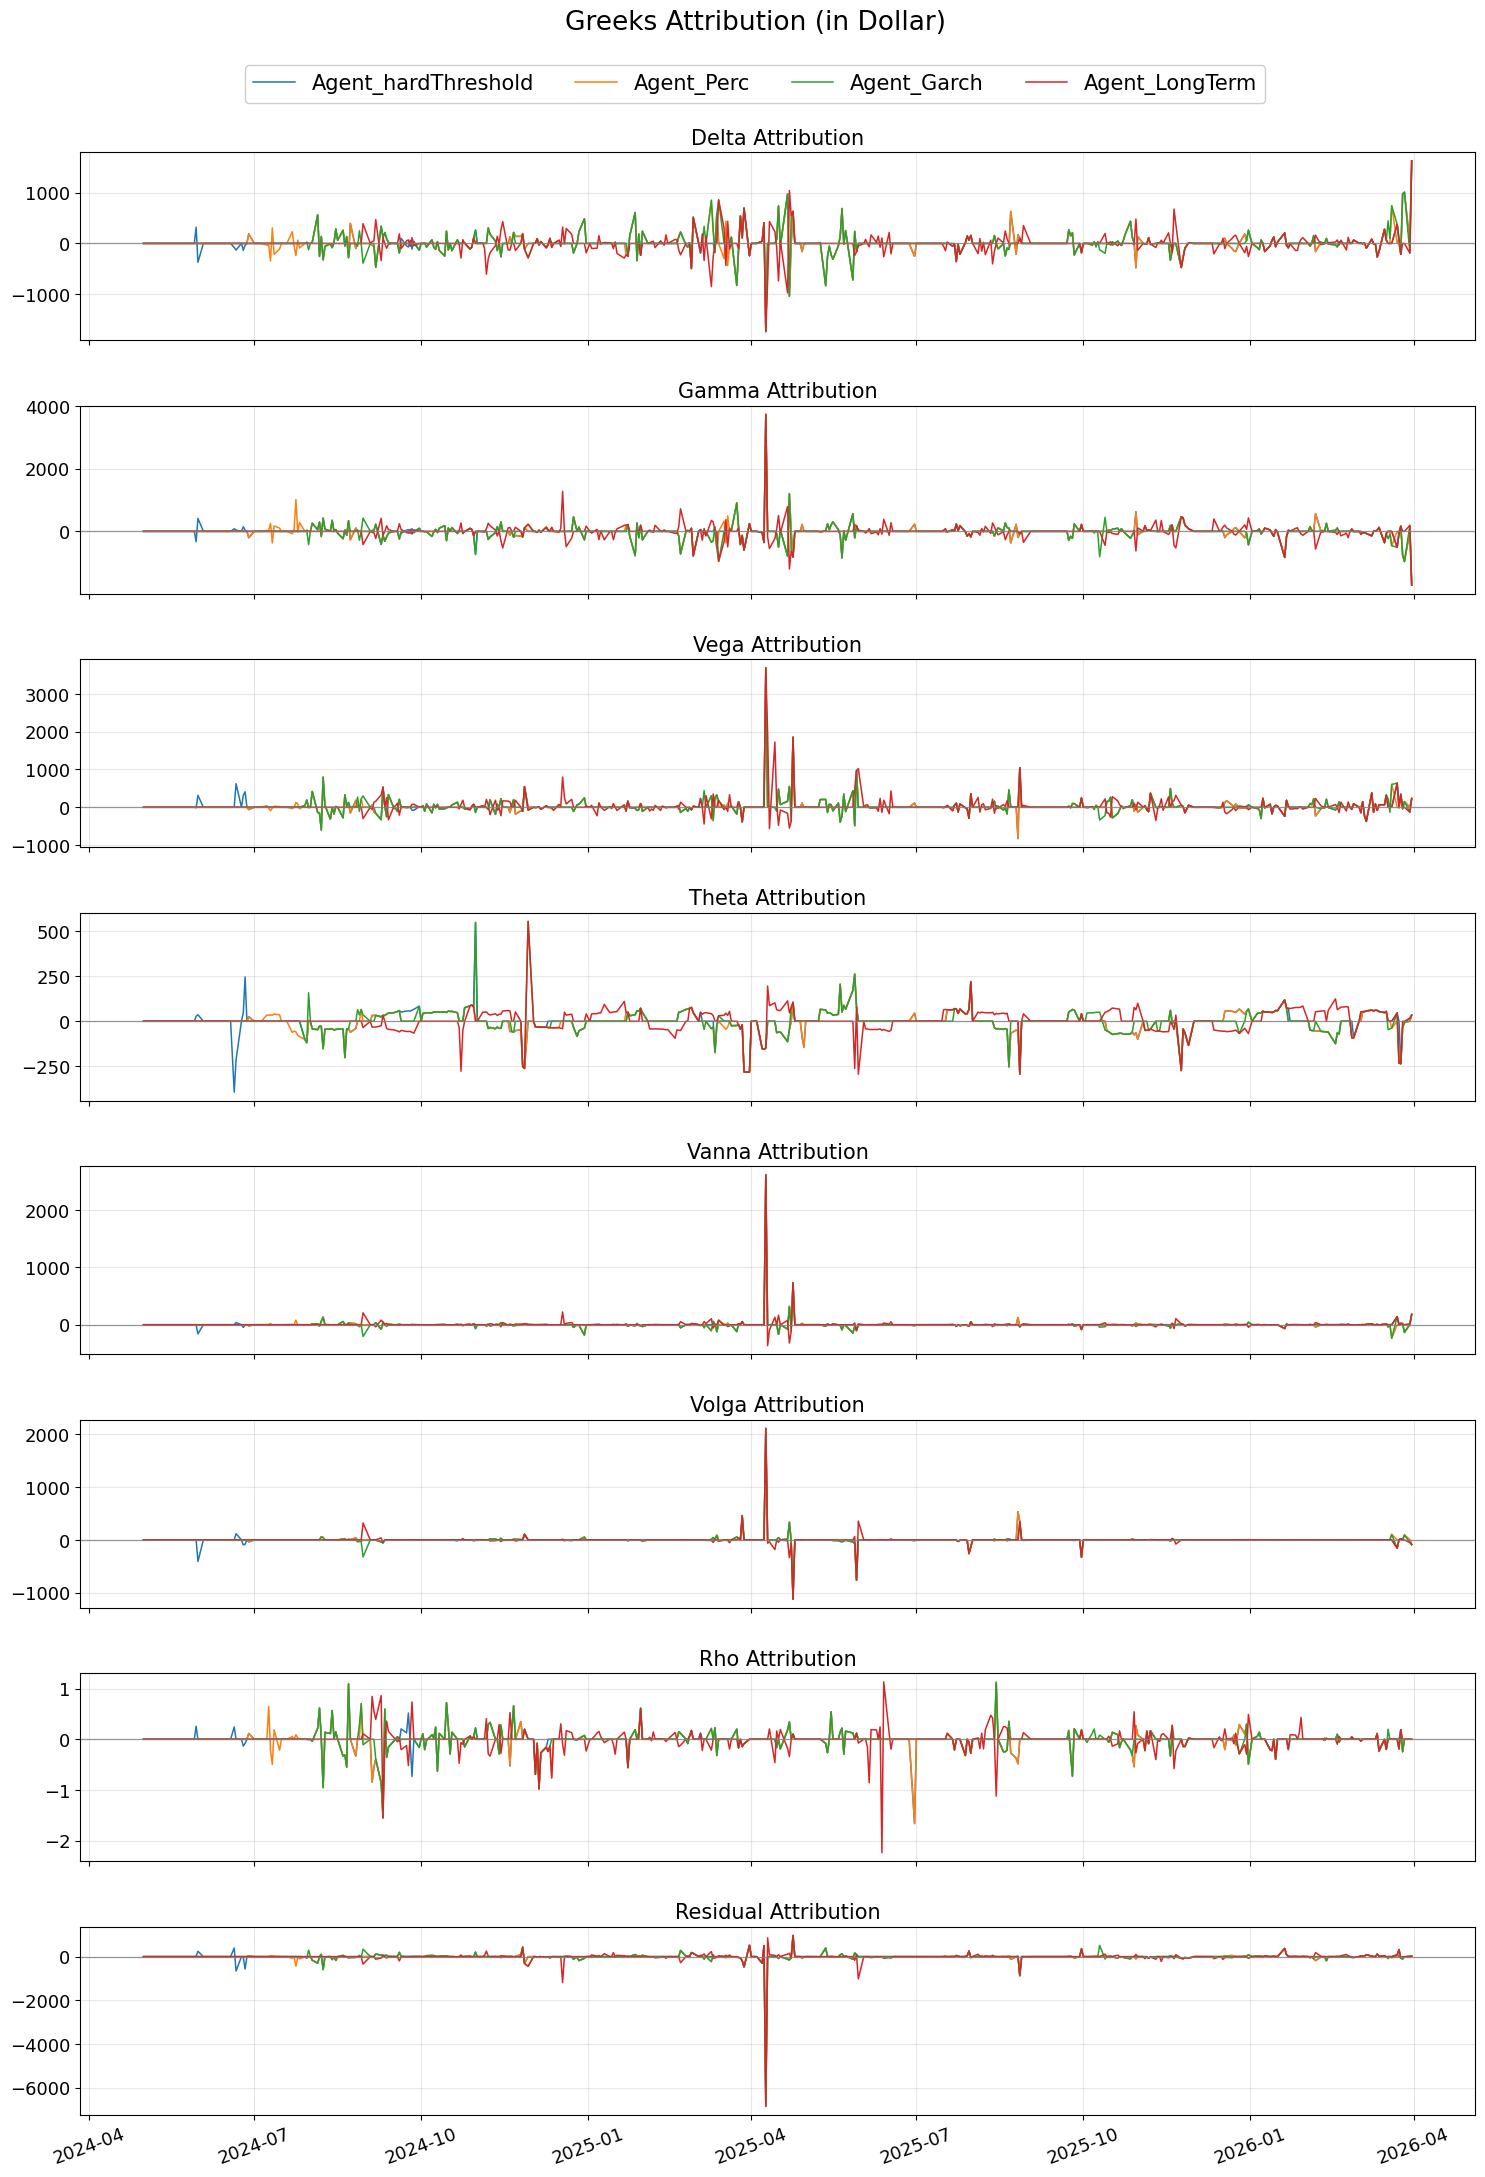
\includegraphics[width=0.70\textwidth]{images/Greeks_line.png}
  \caption{Greeks exposure over time for each agent on SPY.}
  \label{fig:greeks-line}
\end{figure}

\section{QQQ: Return and Greeks}
\label{app:qqq-return-greeks}

Figure~\ref{fig:qqq-return} and Figure~\ref{fig:qqq-greeks} report the return and Greeks diagnostics for QQQ.

\begin{figure}[H]
  \centering
  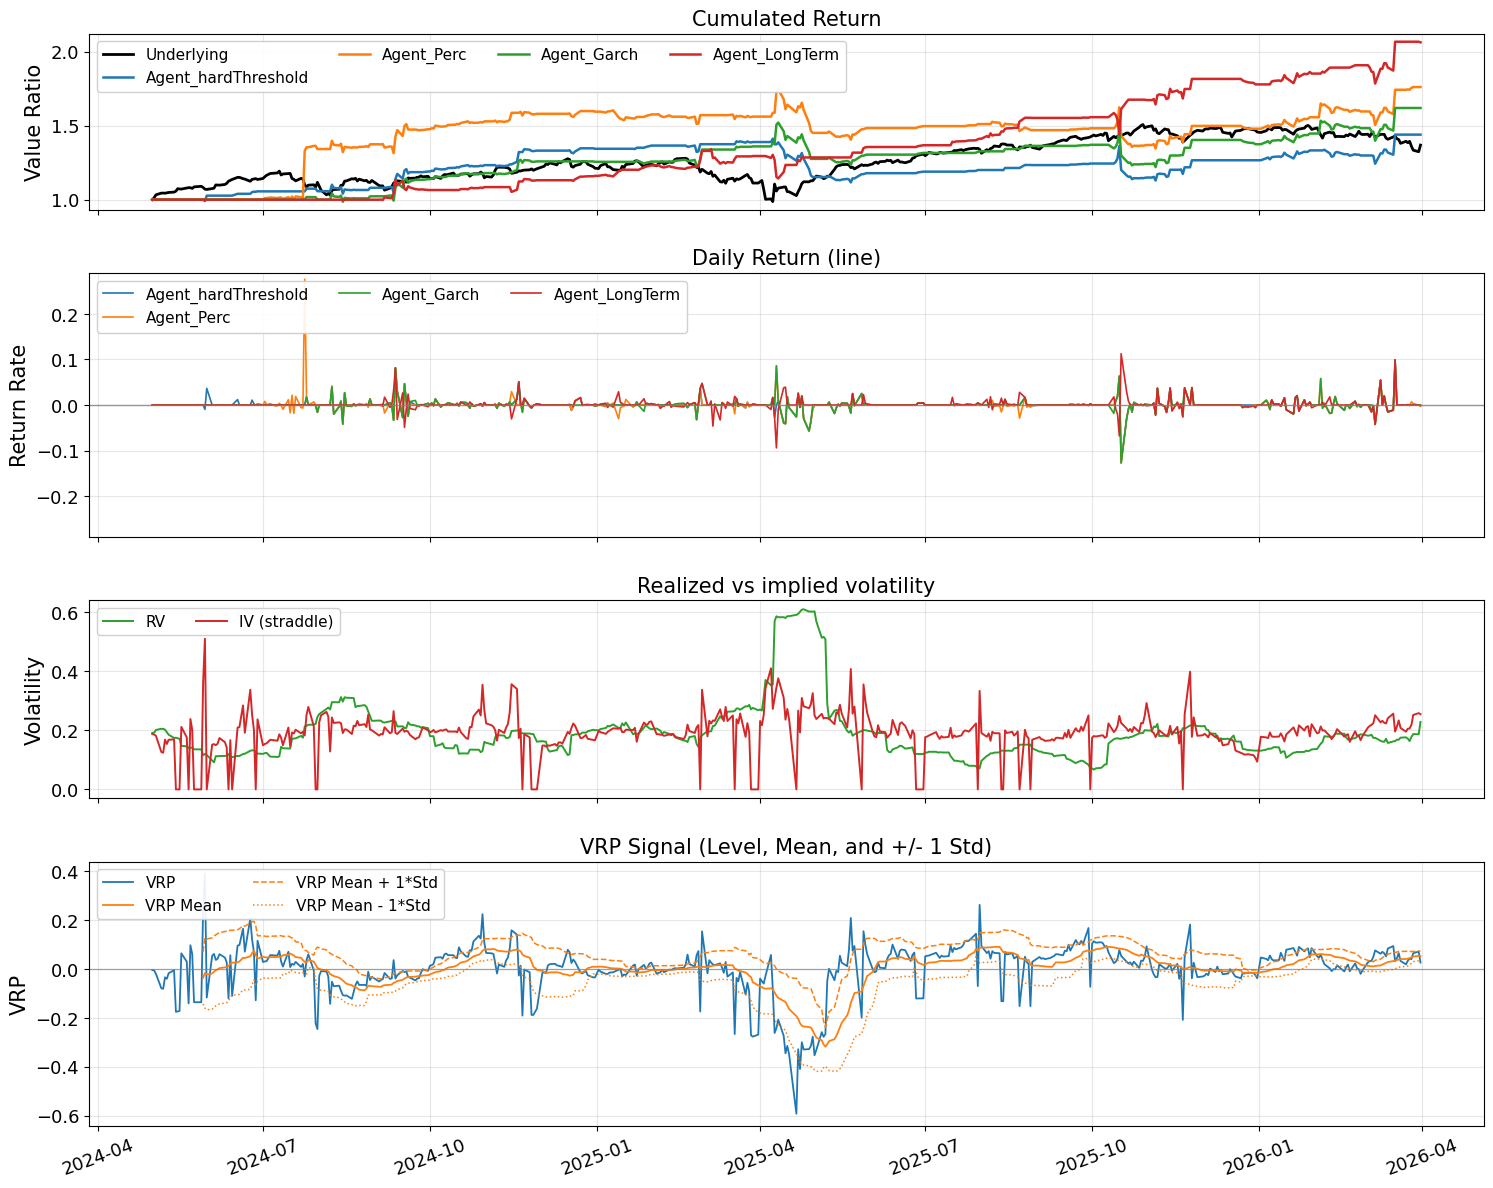
\includegraphics[width=0.85\textwidth]{images/QQQ_return.png}
  \caption{QQQ return diagnostics.}
  \label{fig:qqq-return}
\end{figure}

\begin{figure}[H]
  \centering
  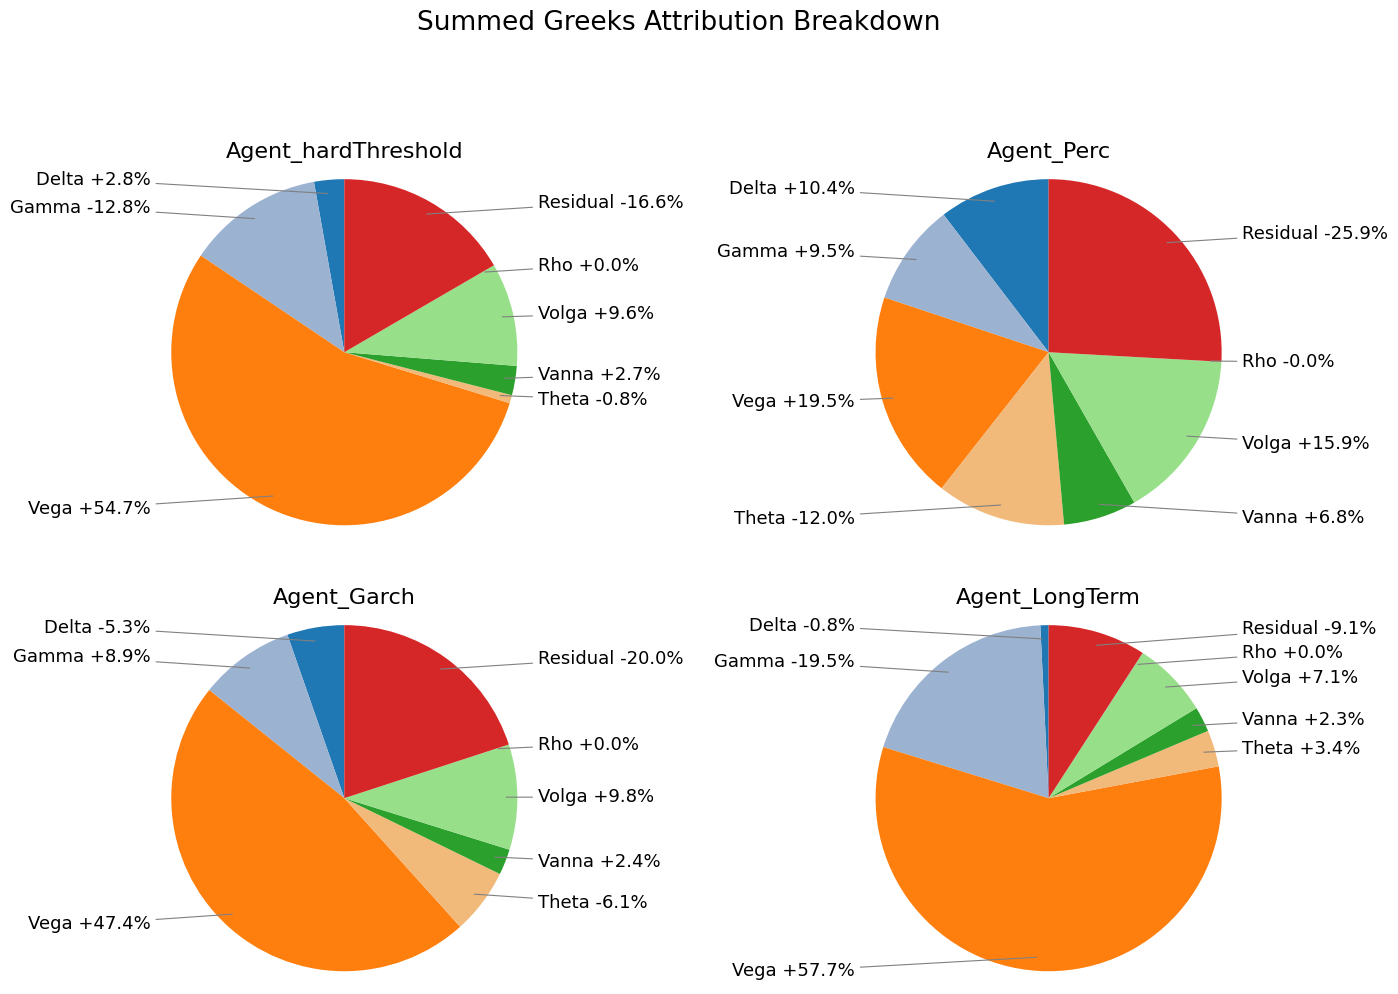
\includegraphics[width=0.75\textwidth]{images/QQQ_greeks.png}
  \caption{QQQ Greeks diagnostics.}
  \label{fig:qqq-greeks}
\end{figure}

\section{DIA: Return and Greeks}
\label{app:dia-return-greeks}

Figure~\ref{fig:dia-return} and Figure~\ref{fig:dia-greeks} report the return and Greeks diagnostics for DIA.

\begin{figure}[H]
  \centering
  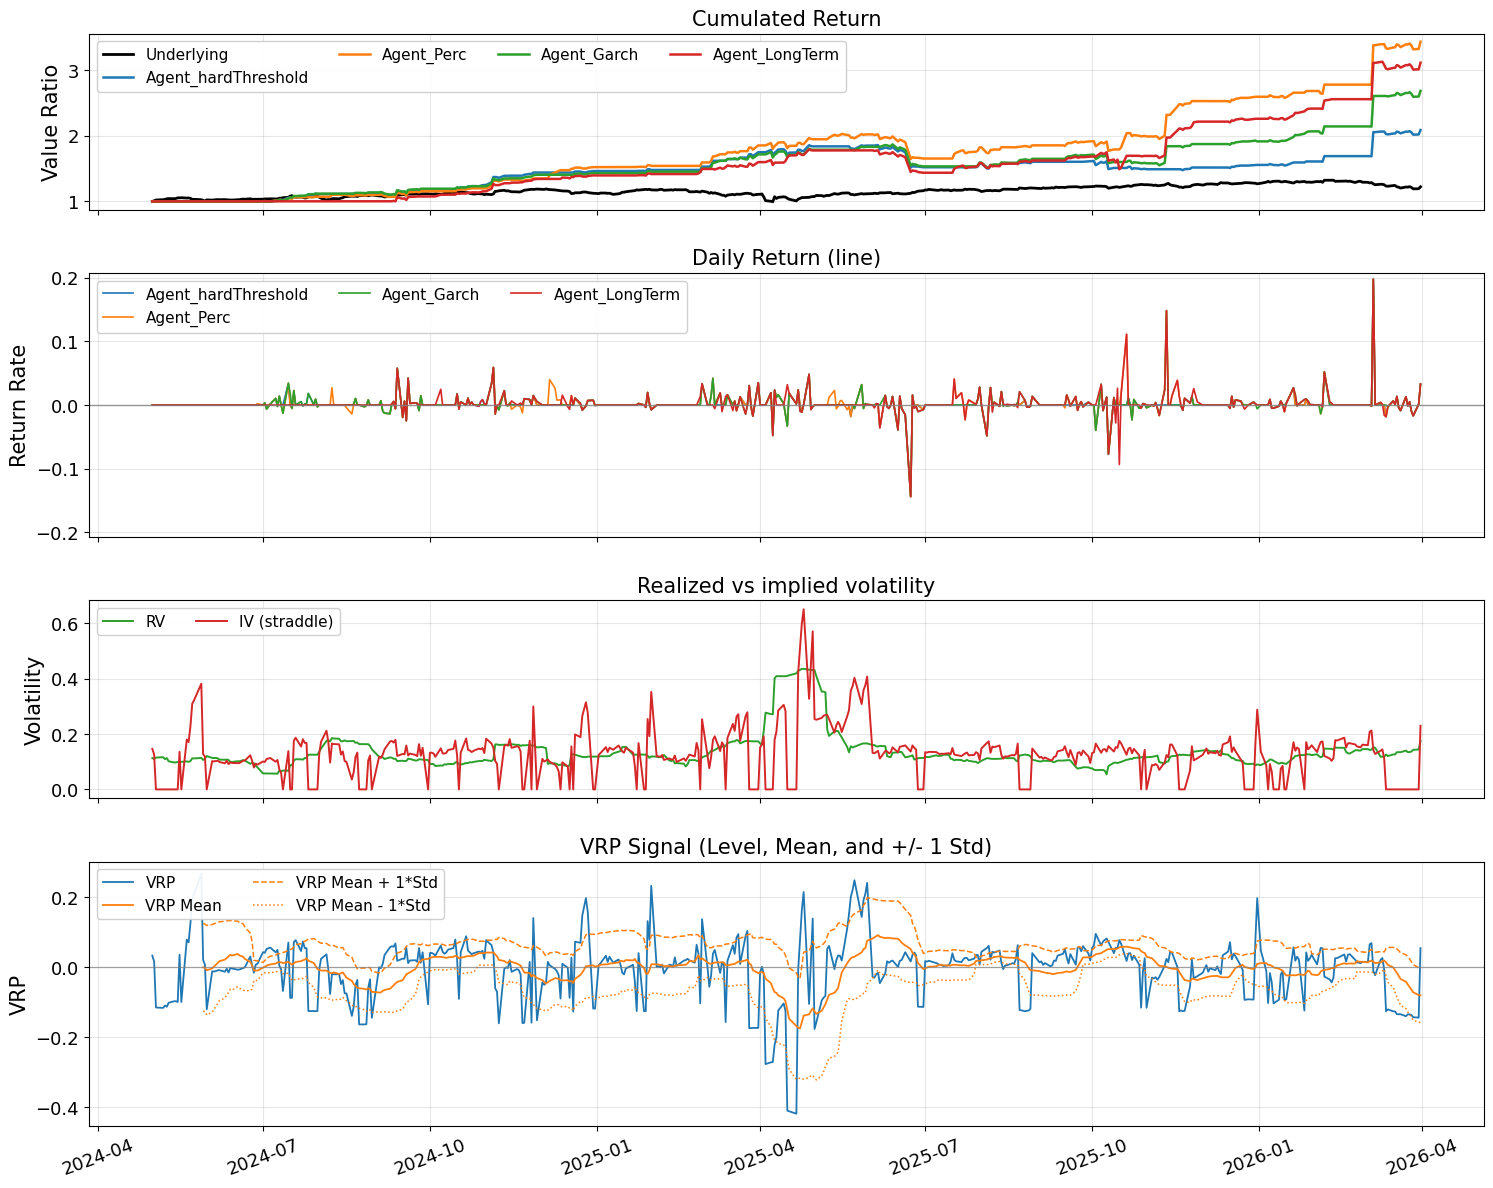
\includegraphics[width=0.85\textwidth]{images/DIA_return.png}
  \caption{DIA return diagnostics.}
  \label{fig:dia-return}
\end{figure}

\begin{figure}[H]
  \centering
  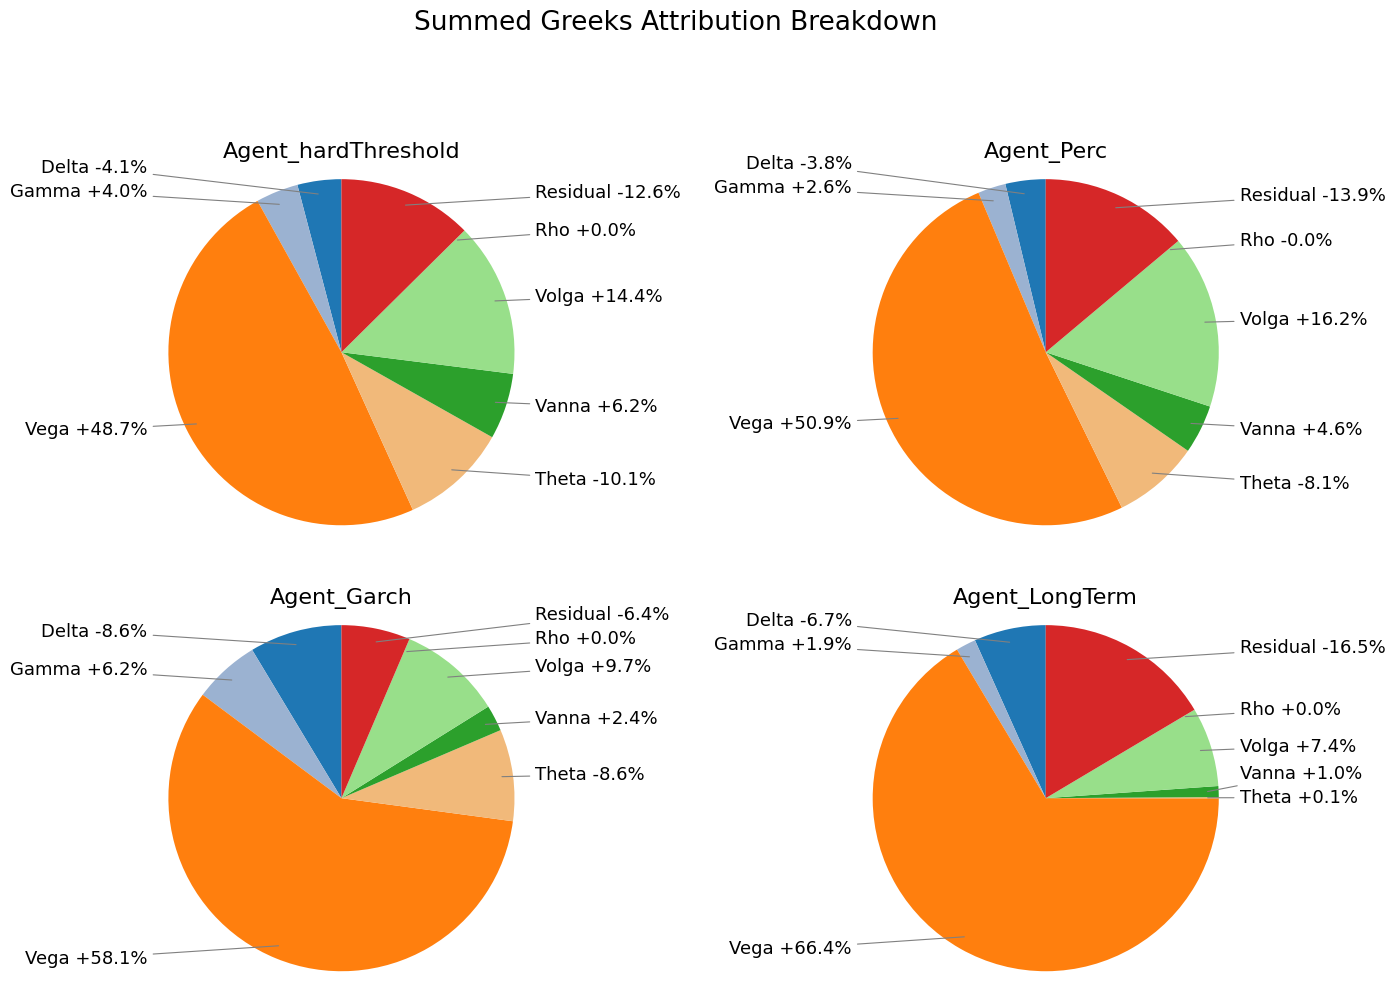
\includegraphics[width=0.75\textwidth]{images/DIA_greeks.png}
  \caption{DIA Greeks diagnostics.}
  \label{fig:dia-greeks}
\end{figure}

\end{document}
